\ParallelTitle{Three ideas explained}{三个概念的学习笔记}
\ParallelText{intro}
 {Learn to calculate a whole-trip average, measure a rectangle, and predict a stack's next output. These are three independent lessons. Read each English paragraph beside its Chinese counterpart; the Quick Reference provides keyword lookup.}
 {学习如何计算全程平均速率、求矩形面积，以及预测栈的下一次输出。这是三个独立的主题。英文在左，中文在右，对应段落并排呈现；配套速查表支持关键词检索。}
\ParallelSection{speed}{Average speed}{平均速率}
\ParallelSubsection[concept]{speed-meaning}{What the average tells you}{平均值的含义}
\ParallelText{speed-definition}
 {Average speed describes an entire time interval. Let $d$ be the total distance travelled and $\Delta t$ the elapsed time, including pauses. Divide distance by time, with $\Delta t>0$:}
 {平均速率描述一整个时间区间。用 $d$ 表示总路程，用 $\Delta t$ 表示总时间，包含停顿。用路程除以时间，且必须满足 $\Delta t>0$：}
\ParallelText{speed-formula}
 {\[v_{\mathrm{avg}}=\frac{d}{\Delta t}\] With metres (m) and seconds (s), the unit is metres per second (m/s). The average alone does not tell you the speed at a particular instant or the maximum speed.}
 {\[v_{\mathrm{avg}}=\frac{d}{\Delta t}\] 路程用米（m）、时间用秒（s）时，速率的单位是米每秒（m/s）。仅凭平均值，无法知道某一瞬间的速率或最高速率。}
\ParallelSubsection[example]{speed-worked}{Worked trip and arithmetic check}{完整行程与计算核验}
\ParallelText{speed-trip}
 {The traveller covers 60 m from A to B, then 120 m from B to C, in 12 s altogether. First add the distances; then divide by the whole elapsed time.}
 {行进者从 A 到 B 走了 60 m，再从 B 到 C 走了 120 m，全程共用 12 s。先把各段路程相加，再除以全程总时间。}
\ParallelText{speed-diagram}
 {\begin{center}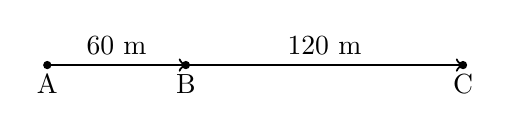
\begin{tikzpicture}[x=0.88cm,y=0.65cm]
 \draw[->,thick] (0,0)--(2,0) node[midway,above]{60 m};
 \draw[->,thick] (2,0)--(6,0) node[midway,above]{120 m};
 \foreach \x/\t in {0/A,2/B,6/C}{\fill (\x,0) circle(1.5pt);\node[below] at (\x,0){\t};}
 \end{tikzpicture}\end{center}\textit{Original schematic of the source trip.}}
 {\begin{center}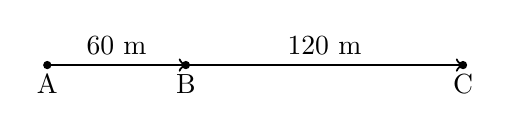
\begin{tikzpicture}[x=0.88cm,y=0.65cm]
 \draw[->,thick] (0,0)--(2,0) node[midway,above]{60 m};
 \draw[->,thick] (2,0)--(6,0) node[midway,above]{120 m};
 \foreach \x/\t in {0/A,2/B,6/C}{\fill (\x,0) circle(1.5pt);\node[below] at (\x,0){\t};}
 \end{tikzpicture}\end{center}根据原材料行程绘制的示意图。}
\ParallelText{speed-calculation}
 {\[\begin{aligned}d&=60+120=180\ \mathrm{m},\\v_{\mathrm{avg}}&=\frac{180\ \mathrm{m}}{12\ \mathrm{s}}=15\ \mathrm{m/s}.\end{aligned}\]
 Check: $(15\ \mathrm{m/s})(12\ \mathrm{s})=180\ \mathrm{m}$. This recovers the distance and checks the arithmetic; it does not establish measurement accuracy.}
 {\[\begin{aligned}d&=60+120=180\ \mathrm{m},\\v_{\mathrm{avg}}&=\frac{180\ \mathrm{m}}{12\ \mathrm{s}}=15\ \mathrm{m/s}.\end{aligned}\]
 核验：$(15\ \mathrm{m/s})(12\ \mathrm{s})=180\ \mathrm{m}$。反算得到原来的路程，可以检查计算过程，但不能证明测量准确。}
\ParallelSubsection[caution]{speed-pitfalls}{Two easy mistakes}{两个常见误区}
\ParallelText{speed-duration}
 {\textbf{Do not average two unequal speeds without checking time.} Here $60/10=6$ s and $120/20=6$ s. The durations are equal, so $(10+20)/2=15$ m/s works. For two unequal speeds, the arithmetic mean equals the trip average only when the durations are equal.}
 {\textbf{两个不同速率不能不看用时就直接取算术平均值。}这里 $60/10=6$ s，$120/20=6$ s。两段用时相等，因此 $(10+20)/2=15$ m/s 成立。对于两个不同的速率，只有两段用时相等，算术平均值才等于全程平均速率。}
\ParallelText{speed-distance}
 {\textbf{Distance is not displacement.} Distance counts the path travelled; displacement compares the finishing position with the starting position. A round trip can have positive distance but zero displacement. Use distance in this formula.}
 {\textbf{路程不等于位移。}路程累计走过的路径长度；位移由起点和终点的位置变化决定。往返行程的路程可以大于零，而位移为零。本公式使用的是路程。}
\ParallelText{speed-gap}
 {\textbf{Source gap:} no method for estimating measurement uncertainty is supplied. No numerical uncertainty can be assigned from this source.}
 {\textbf{原材料的缺口：}没有提供测量不确定度的估计方法，因此不能据此给出数值化的不确定度。}
\clearpage
\ParallelSection{area}{Rectangle area}{矩形面积}
\ParallelSubsection[concept]{area-meaning}{Counting unit squares}{数单位正方形}
\ParallelText{area-definition}
 {Area measures a two-dimensional region. One square metre is the area of a square with sides of 1 m. A rectangle 3 m wide and 2 m high holds six such squares, with no gaps or overlaps.}
 {面积度量二维区域的大小。1 平方米是边长为 1 m 的正方形的面积。一个宽 3 m、高 2 m 的矩形，可以由六个这样的正方形铺满，既无空隙，也不重叠。}
\ParallelText{area-diagram}
 {\begin{center}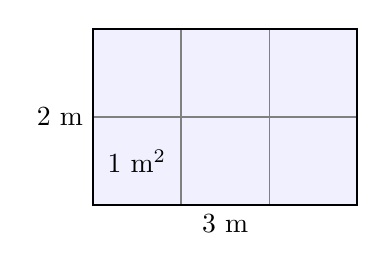
\begin{tikzpicture}[x=1.12cm,y=1.12cm]
 \fill[blue!6] (0,0) rectangle(3,2);
 \draw[step=1,gray] (0,0) grid(3,2);
 \draw[thick] (0,0) rectangle(3,2);
 \node[below] at(1.5,0){3 m};\node[left] at(0,1){2 m};
 \node at(.5,.5){$1\ \mathrm{m^2}$};
 \end{tikzpicture}\end{center}\textit{Original drawing: three columns of two unit squares.}}
 {\begin{center}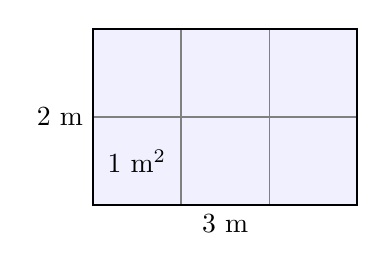
\begin{tikzpicture}[x=1.12cm,y=1.12cm]
 \fill[blue!6] (0,0) rectangle(3,2);
 \draw[step=1,gray] (0,0) grid(3,2);
 \draw[thick] (0,0) rectangle(3,2);
 \node[below] at(1.5,0){3 m};\node[left] at(0,1){2 m};
 \node at(.5,.5){$1\ \mathrm{m^2}$};
 \end{tikzpicture}\end{center}原创图示：三列，每列两个单位正方形。}
\ParallelText{area-formula}
 {For positive rectangle side lengths $w$ and $h$, \[A=wh,\qquad w>0,\ h>0.\] Thus $(3\ \mathrm{m})(2\ \mathrm{m})=6\ \mathrm{m^2}$. The rule also works for non-integer side lengths.}
 {对于边长为正数的矩形，设宽为 $w$、高为 $h$，则 \[A=wh,\qquad w>0,\ h>0.\] 所以 $(3\ \mathrm{m})(2\ \mathrm{m})=6\ \mathrm{m^2}$。边长不是整数时，这一规则仍然适用。}
\ParallelSubsection[example]{area-units}{Convert before multiplying}{先统一单位再相乘}
\ParallelText{area-conversion}
 {A length of 200 cm equals 2 m. For sides 3 m and 200 cm, convert first: \[200\ \mathrm{cm}=2\ \mathrm{m},\qquad A=3\times2=6\ \mathrm{m^2}.\] Writing $3\times200=600\ \mathrm{m^2}$ ignores the incompatible length units. Check that both input lengths use the same unit, and square that unit in the area.}
 {200 cm 等于 2 m。对于边长为 3 m 和 200 cm 的矩形，先换算：\[200\ \mathrm{cm}=2\ \mathrm{m},\qquad A=3\times2=6\ \mathrm{m^2}.\] 写成 $3\times200=600\ \mathrm{m^2}$，就忽略了长度单位不一致的问题。检查两个边长是否使用同一单位，面积的单位应为该长度单位的平方。}
\ParallelSubsection[concept]{area-scaling}{How scaling changes area}{缩放如何改变面积}
\ParallelText{area-scale-rule}
 {Scale both side lengths by the same positive factor $k$. The new area is \[A'=(kw)(kh)=k^2wh=k^2A.\] Doubling just one side doubles the area. Doubling both sides multiplies it by four. For the 3 m by 2 m rectangle, the derived examples are $6\times2=12\ \mathrm{m^2}$ and $6\times4=24\ \mathrm{m^2}$.}
 {把两个边长都乘以同一个正数 $k$，新面积就是 \[A'=(kw)(kh)=k^2wh=k^2A.\] 只把一条边加倍，面积加倍；两条边都加倍，面积变成原来的四倍。由 3 m 乘 2 m 的矩形可推得：$6\times2=12\ \mathrm{m^2}$，$6\times4=24\ \mathrm{m^2}$。}
\ParallelSubsection[caution]{area-boundary}{Choose the right quantity and shape}{分清量与图形}
\ParallelText{area-perimeter}
 {\textbf{Covering a surface needs area; edging it needs perimeter.} Perimeter counts the boundary length: $P=2(w+h)=2(3+2)=10$ m here. It is measured in metres, not square metres.}
 {\textbf{铺满表面要算面积；沿边铺设要算周长。}周长是边界的总长度：本例中 $P=2(w+h)=2(3+2)=10$ m。其单位是米，而不是平方米。}
\ParallelText{area-limitation}
 {\textbf{Shape matters.} Two adjacent side lengths do not by themselves determine the area of an arbitrary quadrilateral. Do not apply the rectangle rule without establishing that the shape is a rectangle.}
 {\textbf{图形的形状很重要。}对于任意四边形，仅知道两条相邻边的长度并不能确定面积。应用矩形面积公式前，要先确认图形确实是矩形。}
\clearpage
\ParallelSection{stack}{Stack behaviour}{栈的行为}
\ParallelSubsection[concept]{stack-meaning}{One accessible end}{只在一端操作}
\ParallelText{stack-definition}
 {A stack adds and removes items at one end, called the \textbf{top}. \textbf{Push} adds an item at the top. \textbf{Pop} removes the top item and returns that item to the caller. The last item put in is the first item taken out: \textbf{last in, first out (LIFO)}.}
 {栈只在同一端添加和移除元素，这一端称为\textbf{栈顶}。\textbf{入栈（push）}把元素放到栈顶；\textbf{出栈（pop）}移除栈顶元素，并把该元素返回给调用者。最后放入的元素最先取出，即\textbf{后进先出（LIFO）}。}
\ParallelText{stack-representation}
 {Write the contents from bottom to top, with the top at the right: $[A,B]$ has $B$ on top. This notation is a description of state, not a required storage layout. Arrays and linked structures can both implement stack behaviour.}
 {这里按从栈底到栈顶的顺序书写，最右边是栈顶：$[A,B]$ 的栈顶为 $B$。这种写法描述的是状态，并不要求某一种存储布局。数组和链式结构都可以实现栈的行为。}
\ParallelSubsection[example]{stack-trace}{Trace the return value and state}{跟踪返回值与状态}
\ParallelText{stack-trace-intro}
 {Start empty. The table follows the exact source sequence. A dash in the return column means that no return value is specified for that push; it does not claim a particular push API.}
 {从空栈开始。下表按原材料给出的顺序逐步执行。返回值一栏中的横线表示原材料未规定入栈操作的返回值，并不指定某一种入栈接口。}
\ParallelText{stack-trace-table}
 {\begin{tabularx}{\linewidth}{@{}l l X@{}}\toprule Operation & Pop returns & State after\\\midrule
 Start & -- & $[\ ]$\\
 Push $A$ & -- & $[A]$\\
 Push $B$ & -- & $[A,B]$\\
 Pop & $B$ & $[A]$\\
 Pop & $A$ & $[\ ]$\\
 Pop & No stored item & Interface-defined\\\bottomrule\end{tabularx}}
 {\begin{tabularx}{\linewidth}{@{}l l X@{}}\toprule 操作 & 出栈返回值 & 操作后状态\\\midrule
 开始 & -- & $[\ ]$\\
 入栈 $A$ & -- & $[A]$\\
 入栈 $B$ & -- & $[A,B]$\\
 出栈 & $B$ & $[A]$\\
 出栈 & $A$ & $[\ ]$\\
 出栈 & 没有已存元素 & 由接口规定\\\bottomrule\end{tabularx}}
\ParallelText{stack-trace-explanation}
 {After pushing $A$ and $B$, the first pop returns $B$ and leaves $[A]$. The second pop returns $A$ and leaves the empty stack. Checking only the returned value is incomplete: also check which items remain.}
 {依次把 $A$ 和 $B$ 入栈后，第一次出栈返回 $B$，剩下 $[A]$；第二次出栈返回 $A$，栈变空。只核验返回值还不够，还要核验剩余元素。}
\ParallelSubsection[caution]{stack-empty}{An empty stack needs a contract}{空栈需要明确约定}
\ParallelText{stack-empty-response}
 {The third pop has no stored item to return. The interface must say what happens, for example an error or an explicit empty result. The source chooses neither response and does not specify an implementation. A test must follow the chosen interface contract rather than assume that pop returns a made-up item.}
 {第三次出栈时，已经没有可返回的已存元素。接口必须明确规定如何处理，例如报错，或返回一个明确表示空的结果。原材料没有选择其中某一种行为，也没有指定实现方式。测试应遵循实际接口约定，而不是假设出栈会返回一个虚构的元素。}
\ParallelSubsection[example]{stack-tests}{Tests that distinguish behaviours}{区分不同语义的测试}
\ParallelText{stack-order-test}
 {\textbf{Removal order:} push $A$, then $B$, then pop. A stack returns $B$ first. A first-in, first-out (FIFO) queue returns $A$ first. The same two inputs therefore distinguish the two removal orders.}
 {\textbf{移除顺序：}先把 $A$ 入栈，再把 $B$ 入栈，然后出栈。栈先返回 $B$；先进先出（FIFO）队列则先返回 $A$。因此，同样的两个输入就能区分这两种移除顺序。}
\ParallelText{stack-capacity-test}
 {\textbf{Capacity:} if the implementation has fixed capacity, separately test what happens when a push would exceed it. Overflow behaviour is not determined by LIFO. The source supplies no specific capacity or overflow response.}
 {\textbf{容量：}如果实现的容量固定，还要单独测试入栈将超出容量时如何处理。后进先出规则并不能决定溢出行为。原材料没有提供具体容量，也没有规定溢出时的响应。}
